\documentclass[12pt]{article} % use larger type; default would be 10pt

\usepackage[utf8]{inputenc} % set input encoding (not needed with XeLaTeX)

\usepackage{graphicx}

\usepackage{listings}
\usepackage[scaled]{beramono}
\usepackage[T1]{fontenc}

\lstset{ basicstyle= \ttfamily, language=Logo, tabsize = 4, showspaces= false, showstringspaces=false}







%%% The "real" document content comes below...

\title{REALLY BIG IMPRESSIVE TITLE}
\author{Andrew Rosen \qquad Brendan Benshoof }
\date{} % Activate to display a given date or no date (if empty),
         % otherwise the current date is printed 

\begin{document}
\maketitle

\section{Problem Space}



\subsection{Chord}

REWRITE THIS AND ADD MORE ABOUT PSUEDOCODE 

Chord \cite{Chord} takes in some key (in this case the hash of a block of data), and returns the identity (ID) of the node responsible for that key.  Both the keys and the nodes are hashed to create an $m$-bit identifier.

Chord takes the nodes and structures them into a circle composed of less than $2^m$ nodes, ordered clockwise by identifier from lowest to highest.  Chord then takes the keys and places each in the node that has the same hashed identifier as it or the node with the first identifier that follows this value.  The node that takes some key $\kappa$ is known as the $successor$ of $\kappa$, or $successor(\kappa)$.  Since we are dealing with a circle, this assignment is done in module $2^m$ space.  For example, if there were some portion of the network with nodes 20, 25, and 27, node 25 would be responsible for the keys [21,22,23,24,25].


With this, we can lookup the node responsible for some key by asking the next node in the circle for the information, who would then pass the request through the circle until the node with the identifier equal or first succeeding the value of the key was found.  That node would be then be able to pass the data, should it exist, back to the requesting node.  This naive approach is largely inefficient, but provides a base example on how nodes in Chord search for information.

What makes Chord efficient is that each node stores the locations of up to $m$ other nodes in the network a \emph{finger table}.  The $i$th entry of the \emph{finger table} of  node $n$ will be the location of $successor(n+2^{i-1})$ $mod$ $2^m$. When a node wants to find some key, it looks to the entry in the finger table that will get it closest to the key without going past.  This allows each step in the to skip up to half the nodes in the network, giving a $\log_2(n)$ lookup time. An example Chord network is shown in Figure \ref{chordreal}.

Further details and the specifics of maintenance and protocol can be found in Stioca et al.'s paper on Chord \cite{Chord}.
ADD SOME MORE PSUEDOCODE


\section{Goals of Modeling and Simulation}
We chose to specifically examine the formation period of a Chord Hash. The cited papers discuss how a single node can join a Chord Hash but gloss over the inital state for building a Chord Hash from scratch in a distributed setting. This made general simulaton of Chord difficult as at least an inital chord ring had to be "boot-strapped" as a pre-connected inital ring so that other nodes can join it. Beause this was an achitecture level design problem, we were not interested in parts of the Chord Hash technique like the behavoir of the actual network topology, latentcy, and server capacity. Thus we make a series of simplifying assumptions.

For this simulation we only consider the over-lay topology, not the underlaying topology of the netowork, thus we create links with the assumption that nodes have the potenital to link into a clique (and in many small netowork cases the system does actually form a clique).

It is important that our latency for this simualtion be varied, but only so that behavoirs that only occur in race conditon could become apparent if they existed but for our purposes the exact qualities of that varience could be left vauge. This allowed us to use travel from node to node in a 2D space


\section{Developed Models}




\begin{lstlisting}
to perform-task
	do-something
end
\end{lstlisting}


\section{Experiments}

\section{Results}

\section{Conclusion and Future Work}



\begin{figure}
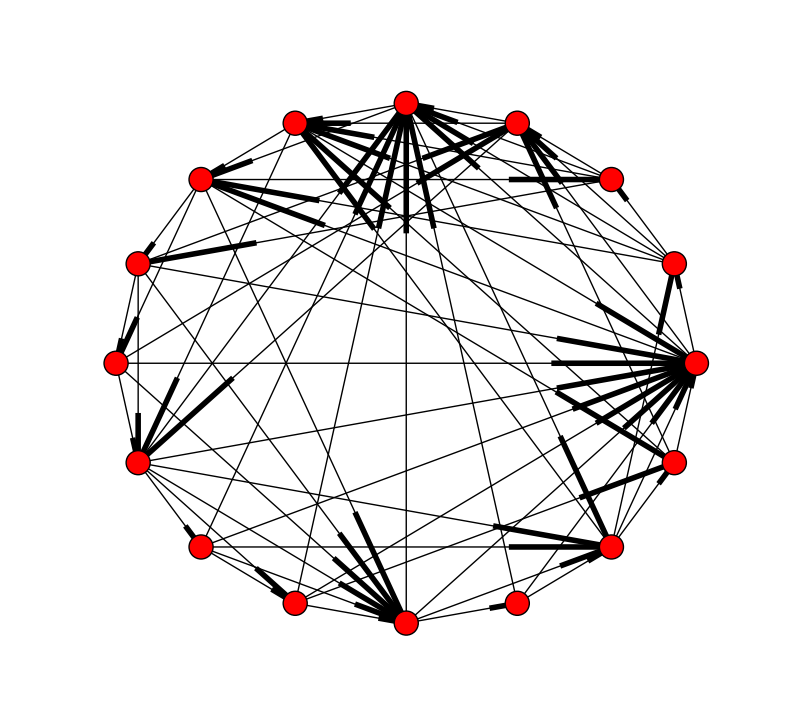
\includegraphics[width=\linewidth]{chordreal}
\caption{An example size 16 network produced by the simulation.  The lines edges are incoming edges.  Note that, unlike in an ideal Chord network, nodes have differing numbers of incoming and outgoing edges.}
\label{chordreal}
\end{figure}






\bibliographystyle{plain}
\bibliography{IRMLP}


\end{document}